\section{Optimization}
  One possible optimization used in the BOTS benchmarks is implementing a cutoff option.
  This can be achieved by using if clause which is provided by the task directive as it is described in \cite{LaGrone.2011}.
  In case this clause evaluates to false no task will be spawned and the execution continues with the function call.
  Figure \ref{fig:cutoff} shows the results without a cutoff and with a cutoff level equal to eight. 
\begin{figure}[h]
	\centering
	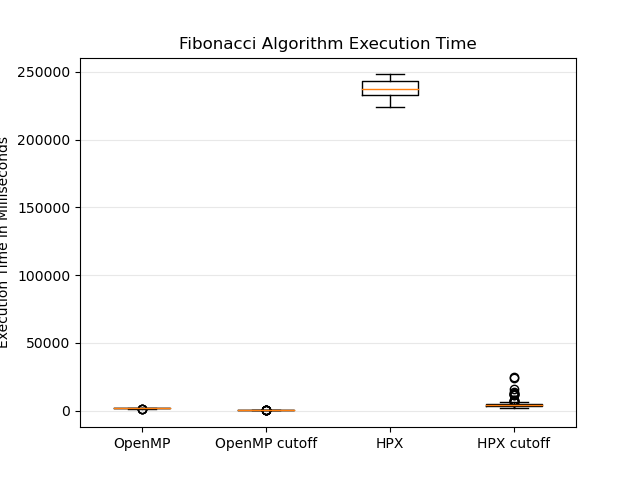
\includegraphics[width=0.45\textwidth]{figures/cutoff_plot.png}
	\caption{Execution times of the Fibonacci algorithm with cutoffs}
	\label{fig:cutoff}
\end{figure}

The mean values of 100 runs are \(2057.34\) ms and \(394.87\) ms for OpenMP without and with a cutoff.
The average measurements for HPX are \(237491.49\) ms without and \(5267.67\) ms with cutoff.
It can be seen that the HPX implementation benefits more by the cutoff.
HPX speeds up by a ratio of approximately \(45\) and the OpenMP implementation speeds up only by \(5\).
 
   
  Another optimization approach might be to see if there is a difference in using tied or untied tasks.
  Untied tasks improve the load balancing as each free thread can start executing a task which is ready to be executed.
  The disadvantage of untied tasks is that the data is not always available locally.
  This means in case a thread wants to execute a ready task which is not created by it, the data and context has to be transferred to new execution location.
  \textbf{TODO: UNTIED VS TIED TASKS}	
	
		
    
    
    \cite{MKlemm.2018}
 --> directives to optimize
 	-->taskyield - suspend the current task in favor of execution of a different task
 	--> if - in case it is false the task is executed immediately
 	--> mergeable - A task for which the data environment, is the same as that of its generating task region
 	--> final - force all child tasks to become final and included
 		--> if true --> child tasks become included --> means that the tasks are also executed by the parent task

  \cite{TheSTEARGroup.2020}
    - HPX --> Performance counters to identify bottlenecks
    - HPX exposes special API functions to allow one to create, manage and read the counter data
    - all performance counter instances have a unique name to access the counter


  \cite{hpxMP.2019}
  \cite{TheSTEARGroup.2020}
    - HPX supports 7 different thread scheduling policies:
      - priority scheduling /default: 1 high priority and 1 low priority queue Queue per OS thread
      - static priority scheduling: 1 low and 1 high prio queue per OS thread --> round robin used in queue
      - local scheduling: 1 queue per per OS thread
      - static scheduling: 1 queue per OS thread --> round robin
      - global scheduling: one shared queue
      - ABP scheduling: double ended lock-free queue per OS thread --> insert threads on top and steal threads from bottom
      - Hierarchy scheduling: tree of task items, each OS Thread traverses through to obtain new task item
      - Periodic priority scheduling: 1 queue of task items per OS thread, couple of high priority queues and one low priority queue
      